{\color{indiagreen}\subsection{Energija nihanja}}
*Idealne razmere(brez upora zraka, vsa nihala nihajo konst. \dots)\\
\begin{align*}
	W &= \text{konst}\\
	W &\dots \text{celotna energija nihanja}\\
\end{align*}
\textbf{Vzmetno nihalo}\\
%\begin{center}
%	\includegraphics[width=15cm, height=15cm,keepaspectratio=true]{EnergijaNihanja.png}
%\end{center}
\begin{align*}
	W &= W_k + W_{pr}\\
	\text{Amplitudna lega}:& W_k = 0, W_{pr0}\\
	{\color{bostonuniversityred}W} &= {\color{bostonuniversityred}W_{pr0}} = {\color{bostonuniversityred}\frac{ks_0^2}{2}}\\
	\text{Ravnovesna lega}:& W_{k0}, W_{pr} = 0\\
	{\color{bostonuniversityred}W} &= {\color{bostonuniversityred}W_{k0}} = {\color{bostonuniversityred}\frac{mv_0^2}{2}}\\
	\text{Poljubna lega}:&\\
	{\color{bostonuniversityred}W} = {\color{bostonuniversityred}W_{pr} + W_{k}} &= {\color{bostonuniversityred}\frac{ks_0^2}{2} + \frac{mv_0^2}{2}}\\
\end{align*}
$t = 0$ desna amplitudna lega.\\
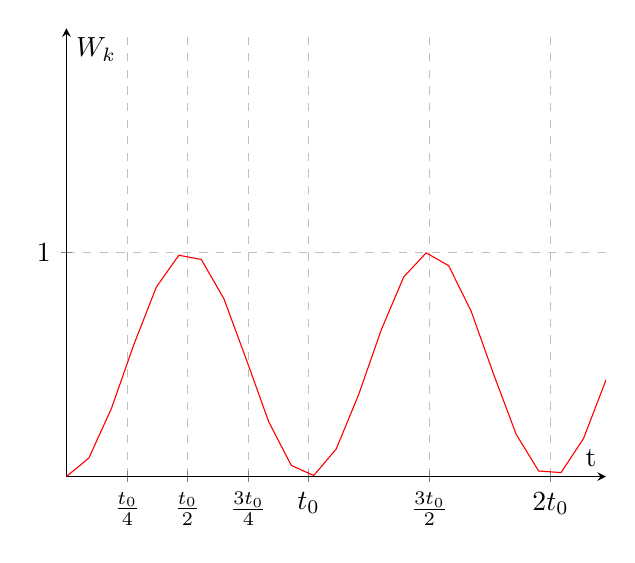
\begin{tikzpicture}
	\begin{axis}[
	    xlabel={t},
	    ylabel={$W_k$},
	    xmin=0, xmax=7,
	    ymin=0, ymax=2,
	    xtick={0,0.79, 1.57, 2.36, 3.14, 4.71, 6.28},
	    ytick={0,1},
	    xticklabels={0,$\frac{t_0}{4}$, $\frac{t_0}{2}$, $\frac{3t_0}{4}$, $t_0$, $\frac{3t_0}{2}$, $2t_0$},
	    ymajorgrids=true,
	    xmajorgrids=true,
	    grid style=dashed,
	    axis lines=middle,
	]
	\addplot[domain=0:7,red] {sin(deg(x))^2};
	\end{axis}
\end{tikzpicture}\\
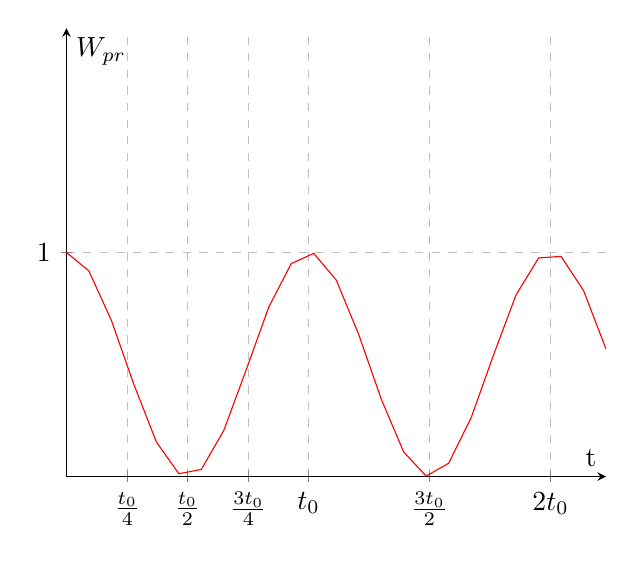
\begin{tikzpicture}
	\begin{axis}[
	    xlabel={t},
	    ylabel={$W_{pr}$},
	    xmin=0, xmax=7,
	    ymin=0, ymax=2,
	    xtick={0,0.79, 1.57, 2.36, 3.14, 4.71, 6.28},
	    ytick={0,1},
	    xticklabels={0,$\frac{t_0}{4}$, $\frac{t_0}{2}$, $\frac{3t_0}{4}$, $t_0$, $\frac{3t_0}{2}$, $2t_0$},
	    ymajorgrids=true,
	    xmajorgrids=true,
	    grid style=dashed,
	    axis lines=middle,
	]
	\addplot[domain=0:7,red] {cos(deg(x))^2};
	\end{axis}
\end{tikzpicture}\\
\begin{tikzpicture}
	\begin{axis}[
	    xlabel={$s_0$},
	    ylabel={$t_0$},
	    xmin=0, xmax=10,
	    ymin=0, ymax=10,
	    xtick={0,2,4,6,8,10},
	    ytick={0,2,4,6,8,10},
	    ymajorgrids=true,
	    xmajorgrids=true,
	    grid style=dashed,
	    axis lines=middle,
	]
	\addplot[domain=0:10,red] {6};
	\end{axis}
\end{tikzpicture}\\
\textbf{Matematično nihalo}\\
%\begin{center}
%	\includegraphics[width=15cm, height=15cm,keepaspectratio=true]{EnergijaNihanja2.png}
%\end{center}
\begin{align*}
	W &= W_p + W_k\\
	\text{Amplitudna lega}:& W_k = 0, W_{p0}\\
	{\color{bostonuniversityred}W} &= {\color{bostonuniversityred}W_{p0}} = {\color{bostonuniversityred}mgh_0}\\
	\text{Ravnovesna lega}:& W_{k0}, W_p = 0\\
	{\color{bostonuniversityred}W} &= {\color{bostonuniversityred}W_{k0}} = {\color{bostonuniversityred}\frac{mv_0^2}{2}}\\
	\text{Poljubna lega}:&\\
	{\color{bostonuniversityred}W} = {\color{bostonuniversityred}W_{p} + W_{k}} &= {\color{bostonuniversityred}mgh_0 + \frac{mv_0^2}{2}}\\
\end{align*}